\section{Перезапуск Handshake}\label{COMMON.Retry} 

Содержание расширения \token[HS.Ext.ks]{key_share}, передаваемого клиентом
в~\token[HS.CH]{ClientHello}, может не устроить сервер. Для ускорения работы
сервер вместо отмены Handshake может продолжить его выполнять при условии
корректировки расширения. Для этого сервер отправляет клиенту
сообщение~\token[HS.HRR]{HelloRetryRequest}, которое включает
\token[HS.Ext.ks]{key_share} с описанием корректировок.
%
Если клиент согласен с корректировками, то он высылает серверу повторное
сообщение \token[HS.CH]{ClientHello} с подправленным расширением, перезапуская
таким образом Handshake (см. рисунок~\ref{Fig.COMMON.Retry}).

\begin{figure}[hbt]
\begin{center}
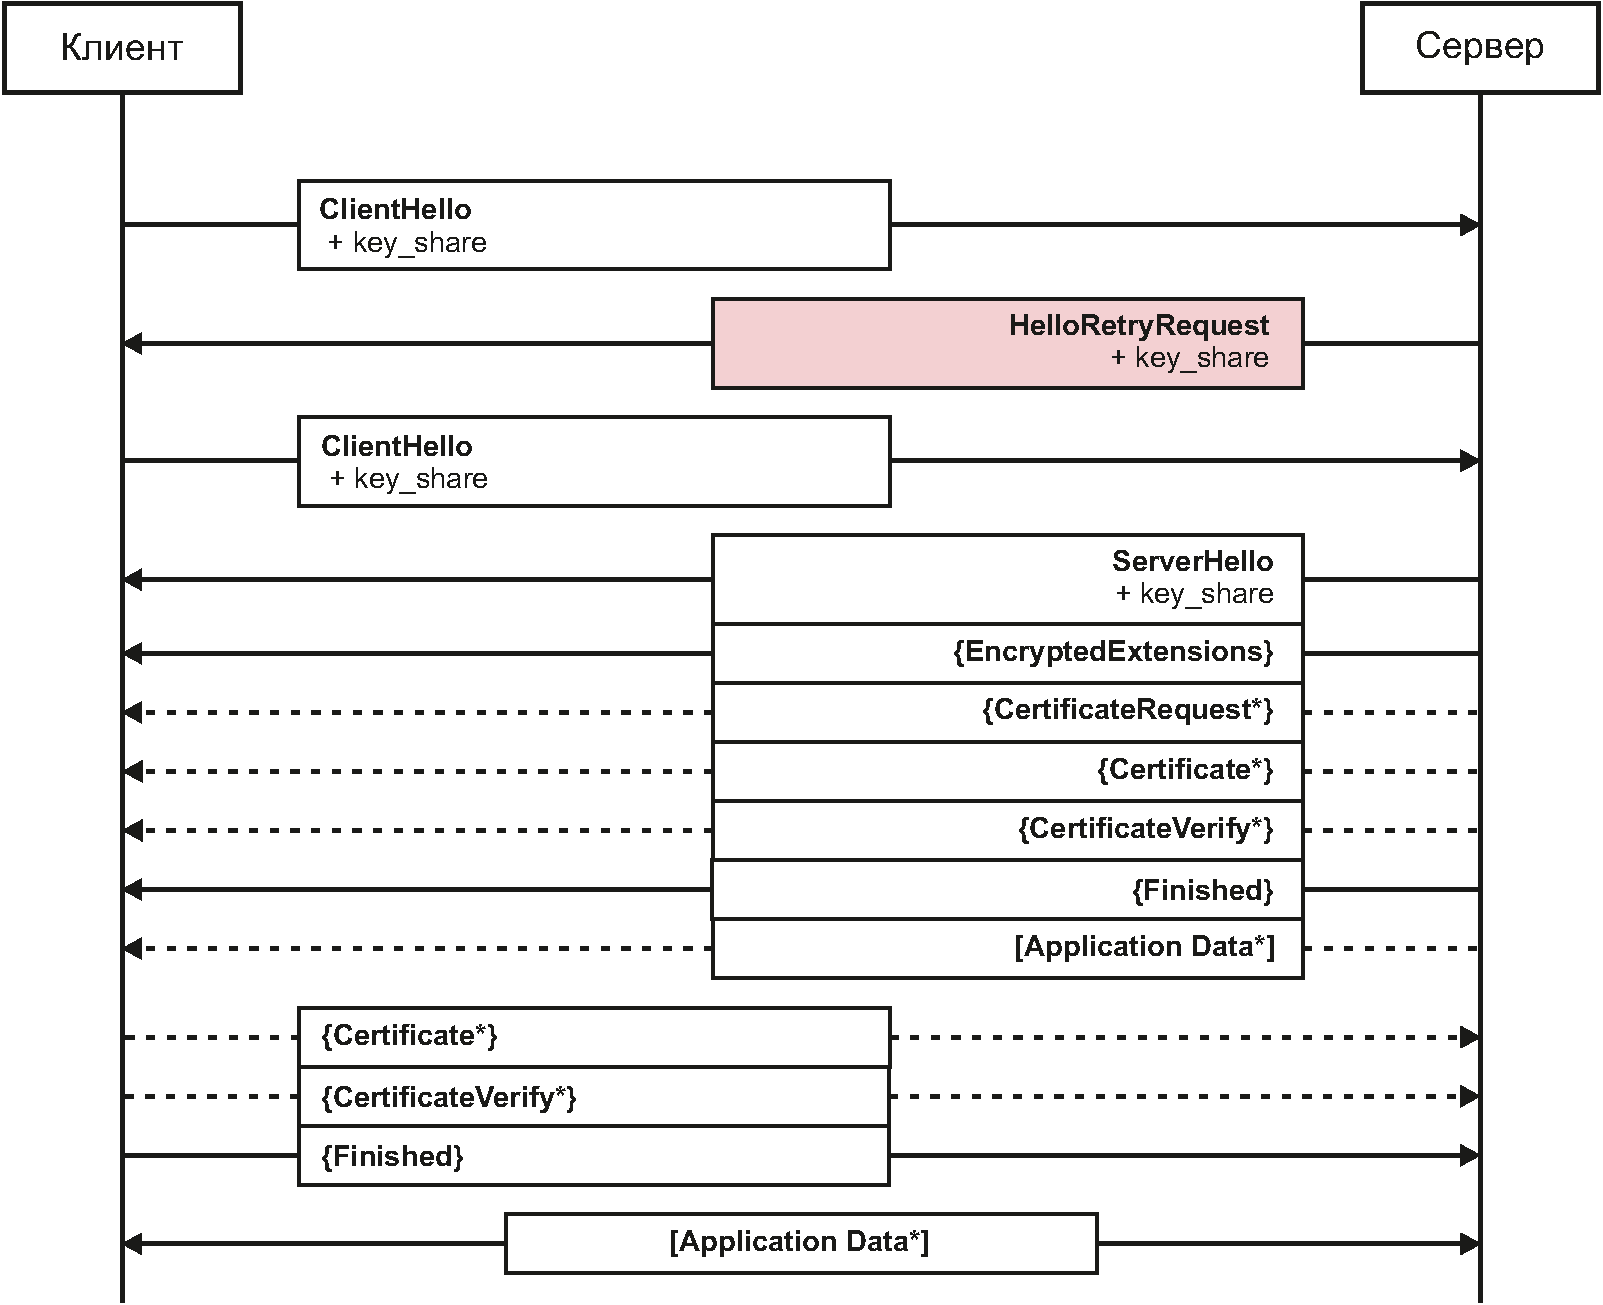
\includegraphics[width=15cm]{../figs/Retry}
\end{center}
\caption{Перезапуск Handshake}\label{Fig.COMMON.Retry}
\end{figure}

Пусть, например, в \token[HS.Ext.ks]{key_share} первого
\token[HS.CH]{ClientHello} перечислены циклические группы режима DHE, ни одна из
которых не устраивает сервер. Тогда сервер указывает допустимую группу в
\token[HS.HRR]{HelloRetryRequest} и клиент использует ее в
повторном~\token[HS.CH]{ClientHello}.

При перезапуске Handshake может выполняться другие корректировки
\token[HS.CH]{ClientHello} (см.~\ref{HS.CH}).

При перезапуске первое сообщение~\token[HS.CH]{ClientHello} и
ответное~\token[HS.HRR]{HelloRetryRequest} остаются в стенограмме Handshake.
